\documentclass[12pt, twoside]{article}

\usepackage{amsfonts}
%\usepackage[T1]{fontenc}
%\usepackage[ansinew]{inputenc}
\usepackage{amssymb}
\usepackage{amsthm}
\usepackage{amsmath}
% \usepackage{ mathrsfs }
\usepackage{dsfont}
\usepackage{natbib}
\setlength{\bibsep}{0pt plus 100ex}
\usepackage{url}
\usepackage{pdflscape}
\usepackage{pdfpages}
\usepackage{svg}
\usepackage[utf8]{inputenc}
\usepackage{graphicx}
\usepackage{bbold}
\usepackage{hyperref}


\usepackage{enumitem}
%\usepackage[german,  onelanguage, linesnumbered]{algorithm2e}
\usepackage{placeins}
\usepackage{a4}
\usepackage[a4paper, ]{geometry}
\geometry{
 a4paper,
 right=30mm,
 left=30mm,
 top=30mm,
 }

% For tables
\usepackage{tabularx}
\usepackage{multirow}
\usepackage{pbox}

% \usepackage{color}

\widowpenalty = 5000
\clubpenalty = 5000


\newcommand{\Prob}{\mathbb{P}}
\newcommand{\V}{\mathbb{V}}
\newcommand{\Cov}{\text{Cov}}
\newcommand{\E}{\mathbb{E}}
\newcommand{\R}{\mathbb{R}}
\newcommand{\N}{\mathbb{N}}
\newcommand{\1}{\mathbb{1}}
\newcommand{\LL}{\mathcal{L}}
\newcommand{\F}{\mathcal{F}}
\newcommand{\iid}{\overset{\text{iid}}{\sim}}
\newcommand{\SUM}{\sum_{i=1}^n}
\newcommand{\PROD}{\prod_{i=1}^n}



\begin{document}

\begin{titlepage}

    \newcommand{\HRule}{\rule{\linewidth}{0.5mm}} % Defines a new command for the horizontal lines, change thickness here

    \center % Center everything on the page
 
    %----------------------------------------------------------------------------------------
    %	HEADING SECTIONS
    %----------------------------------------------------------------------------------------
    
\includegraphics[scale = 0.22]{campus-seal.jpg}\\[0.5cm]
    
     \textsc{\large University of California, Los Angeles}\\[0.2cm] % Minor heading such as course title
     \textsc{\large Department of Statistics}\\[0.5cm]
    %----------------------------------------------------------------------------------------
    %	TITLE SECTION
    %----------------------------------------------------------------------------------------

    \HRule \\[0.4cm]
    { \huge \bfseries Potts Models}\\[0.2cm] % Title of your document
    \HRule \\[0.4cm]
    \textsc{\large Multiple Imputation of Missing Values % Using Swendsen-Wang
    }\\[2.0 cm]
 
    %----------------------------------------------------------------------------------------
    %	AUTHOR SECTION
    %----------------------------------------------------------------------------------------
    
    \hspace{1cm}
    \begin{minipage}{0.4\textwidth}
    \begin{flushleft} \large
    \emph{Author:}\\
        Thomas \textsc{Maierhofer}\\
        SID 905078249 % Your name
    \end{flushleft}
    \end{minipage}
    ~
    \begin{minipage}{0.4\textwidth}
    \begin{flushright} \large
    \emph{Stats 202C:} \\
    Prof. Mark Handcock \\ % Supervisor's Name
    \text{}
    \end{flushright}
    \end{minipage}\\[2cm]
    
    \large{
    Final Project Report
    } \\[2cm]
    
    {\large Spring Quarter 2019,} \\
    {\large June 14, 2019}\\[2cm] % Date, change the \today to a set date if you want to be precise

    %----------------------------------------------------------------------------------------

    \vfill % Fill the rest of the page with whitespace

\end{titlepage}

%\newpage
%\hspace{5cm}
%\newpage

\pagenumbering{roman}
\tableofcontents 
\clearpage

\begin{abstract}
Potts models are a well studied subject of statistical mechanics. This introduces a novel Markov Chain Monte Carlo approach for estimating the joint distribution of missing values in a Potts model. The Swendsen Wang algorithm is used to increase computational efficiency.
\end{abstract}
\clearpage
\pagenumbering{arabic}

\section{Introduction}
The Potts model describes a system of interacting spins on a crystalline lattice. Its predecessor, the Ising model  was originally described in \cite{lenz1920beitrage} to model 
atomic spins
% behavior of positively or negatively charged magnetic needles
and was solved for the 2 dimensional case by \cite{onsager1944crystal}. 
In its generalization for more than two classes, the Potts model is often interpreted as an image, where every point in the lattice is a pixel taking one color in a discrete set.
Usually, all pixels are assumed to be fully observed, which is not necessarily the case in non-experimental settings.
This project proposes a method for estimating the joint distribution of missing pixels in a Potts model of unknown temperature which is based on a Markov Chain Monte Carlo (MCMC) algorithm.

The remainder of this report is structured as follows: Section~\ref{potts_model} formally introduces the Potts model, 
outlines strategies for estimating the inverse temperature and based on this,
sampling from a completely observed Potts models given the inverse temperature. Subsequently, a new method is proposed for estimating the joint distribution of missing values in a Potts model using multiple imputation.
% TODO simulation study
The report concludes in an outlook on unanswered questions for future research (Section~\ref{future_research}).


% \section{Background}
%\subsection{Ising Model}
% \subsection{Markov Chain Monte Carlo}



\clearpage
\section{Potts Model}\label{potts_model}
The Potts model is a direct generalization of the Ising model where the class labels (or spin directions) take $L \in \{2, 3, 4, \ldots\}$ possible values. 
See topright and bottomleft of Figure~\ref{fig:potts_models} for an example of a four class Potts model in equilibrium.
The probability of a given $N \times N$ dimensional lattice $X = (X)_{ij},\ i, j = 1, \ldots, N,$ taking values $x = (x)_{ij} \in \mathfrak X := \{1, 2, \ldots, L\}^{N \times N},$ is given as
\begin{equation}
P(X = x | \beta) = \frac{1}{C(\beta)} \exp \left(-\beta \sum_{i = 1}^N \sum_{j = 1}^N \sum_{(k,l) \in E_{ij}} \1 \{x_{ij} = x_{kl}\}\right),
\end{equation}
where $\beta = 1 / (k T)$ is the inverse temperature $T$ with Boltzmann constant $k$, $C(\beta)$ is the integration constant ensuring that $P(X|\beta)$ is a proper probability distribution
\begin{equation} \label{eq:cbeta}
C(\beta) = \sum_{x \in \mathfrak X} \exp \left(-\beta \sum_{i = 1}^N \sum_{j = 1}^N \sum_{(k,l) \in E_{ij}} \1 \{x_{ij} = x_{kl}\}\right), 
\end{equation}
$E_{ij}$ is the set of all indices sharing an edge with $X_{ij}$, i.e.\ the indices $\{(i + 1, j), (i - 1, j), (i, j + 1), (i, j - 1)\}$, and $\1\{\cdot\} \in\{0, 1\}$ the indicator function which is $1$ if $\cdot$ is true. Note that for notational simplicity the lattice is assumed to be a torus, i.e.\ the pixels $X_{1j}$ share an edge with $X_{Nj}$ and the pixels $X_{i1}$ share an edge with $X_{iN}$ for al $i, j$, and $\mathfrak X$ is the set of all possible colorings $\{1, 2, \ldots, L\}^{N \times N}$ of size $|\mathfrak X| = L^{N^2}$.

The remainder of this section discusses two complementary approaches to the estimation of the inverse temperature $\beta$ in a 2D Potts model in Section~\ref{temperature_estimation}, a pseudlikelihood estimator in Section~\ref{MPLE_estimator} and an MCMC estimator in Section~\ref{MCMC_estimator}. Section~\ref{model_sampling} introduces a Gibbs Sampler (Section~\ref{gibbs_sampler}) and the Swendsen Wang algorithm (Section~\ref{swendsen_wang}) for sampling new observations from a Potts model.
Section~\ref{treatment_of_missing_values} discusses how to use these algorithms to estimate the temperature (Section~\ref{missing_values_temperature}) and sample over missing observations from a partially observed grid (Section~\ref{missing_values_model_sampling}).

\subsection{Temperature Estimation}\label{temperature_estimation}
An important problem arising in Potts models is the estimation of the inverse temperature $\beta$. As there are no feasible analytical results, a maximum pseudolikelihood estimator (MPLE) (Section~\ref{MPLE_estimator}), see e.g.\ \cite{levada2009pseudo}, and a MCMC estimator (Section~\ref{MCMC_estimator}) are used. The MPLE estimator is computationally way more efficient (scaling with $N^2 \cdot L$) than the MCMC algorithm (scaling with $M \cdot N^2 \cdot L$, where $M$ is the number of MCMC samples drawn) but can be biased, particularly for large $\beta$. The MCMC algorithm has the disadvantage that it requires a prespecified starting value $\beta_0^\text{MCMC},$ which needs to be close to the true $\beta$ for the estimator to converge within a practical number of MCMC iterations $M$. The strengths of these two approaches can be combined, by using the MPLE estimator to obtain an initial starting value for the MCMC algorithm,
\begin{equation*}
\beta_0^\text{MCMC} \leftarrow \hat \beta^\text{MPLE},
\end{equation*}
which allows the MCMC algorithm to converge within a reasonable time.


\subsubsection{Maximum Pseudolikelihood Estimator}\label{MPLE_estimator}
The likelihood function for $X$ does can not be factored into likelihood functions for the individual $X_{ij}$, as the distribution of $X_{ij}$ depends on its neighbors $X_{lk}, (l,k) \in E_{ij}$.
Ignoring this dependence, a pseudolikelihood estimator can be obtained, which approximates the true likelihood
\begin{eqnarray}
\LL(\beta | X) &=& P(X = x | \beta) \nonumber \\
&=& \frac{1}{C(\beta)} \exp \left(-\beta \sum_{i = 1}^N \sum_{j = 1}^N \sum_{(k,l) \in E_{ij}} \1 \{x_{ij} = x_{kl}\} \right) \nonumber \\
&=& \prod_{i = 1}^N \prod_{j = 1}^N \frac{1}{C(\beta)} \exp\left(-\beta \sum_{(k,l) \in E_{ij}} \1 \{x_{ij} = x_{kl}\}\right)
\end{eqnarray}
with integration constant $C(\beta)$ given in Equation~\eqref{eq:cbeta},
by the pseudolikelihood
\begin{eqnarray}
\LL^*(\beta | X) &=& \prod_{i = 1}^N \prod_{j = 1}^N P\big(X_{ij} = x_{ij} | \beta, X \setminus X_{ij}\big) \nonumber \\
&=& \prod_{i, j} P\big(X_{ij} = x_{ij} | \beta, X_{kl}\big), \text{ given all }(k, l) \in E_{ij} \nonumber \\
&=& \prod_{i, j} \frac{1}{C_{ij}(\beta)} \exp\left(-\beta \sum_{(k,l) \in E_{ij}} \1 \{x_{ij} = x_{kl}\}\right),
\end{eqnarray}
with integration constant
\begin{equation} \label{eq:cbeta_ij}
C_{ij}(\beta) = \sum_{y = 1}^L \exp\left( -\beta \sum_{(k, l) \in E_{ij}} \1\{x_{kl} = y\}\right).
\end{equation}
The pseudolikelihood estimator is based on the (incorrect) assumption that the neighborhood of every $X_{ij}$ is given and fixed. Additionally to allowing the factorization of the likelihood, the integration constant is simplified dramatically. Instead of summing over all $L^{N^2}$ possible lattices $x \in \{1, \ldots, L\}^{N\times N}$, we only have to sum over all $LN^2$ possible values $x_{ij} \in \{1, \ldots, L\}$ given their fixed neighborhood $E_{ij}$.
%
The maximum pseudolikelihood estimator is obtained maximizing the log-pseu\-do\-likeli\-hood w.r.t.\ $\beta$
\begin{eqnarray}
\ell^*(\beta | X) &=& \log \Big(\LL^*(\beta | X) \Big) \nonumber \\
&=& \sum_{i = 1}^N \sum_{j = 1}^N \log \left(\frac{1}{C_{ij}(\beta)} \exp \Big(-\beta \sum_{(k,l) \in E_{ij}} \1 \{x_{ij} = x_{kl}\}\Big) \right) \nonumber \\
&=& \sum_{i, j} -\log \left( \sum_{y = 1}^L \exp\Big(- \beta \sum_{(k,l) \in E_{ij}} \1\{x_{kl} = y\}\Big) \right) \nonumber\\
&& -  \beta \sum_{i, j} \sum_{(k,l) \in E_{ij}} \1 \{x_{ij} = x_{kl}\} \nonumber \\
&=:& -\sum_{i, j} \log \left( \sum_{y = 1}^L \exp\big(- \beta U_{ij}(y)\big) \right) -  \beta \sum_{i, j} U_{ij}(x_{ij}),
\end{eqnarray}
introducing the notational abbreviation
$$ U_{ij}(y) = \sum_{(k,l) \in E_{ij}} \1 \{x_{kl} = y\} $$
for counts of class $y$ in the neighborhood of $X_{ij}$.
Maximization of the pseudolikelihood is achieved by equating its derivative w.r.t.\ $\beta$ to $0$,
\begin{eqnarray}
\frac{d}{d \beta} \ell^*(\beta | X) &=& -\sum_{i, j} \frac{\sum_{y = 1}^L \exp\big(- \beta  U_{ij}(y)\big) \big(- U_{ij}(y)\big)}{\sum_{y = 1}^L \exp(- \beta  U_{ij}(y)\big)} - \sum_{i, j}  U_{ij}(x_{ij}) \nonumber \\
&\overset{!}{=}& 0 \nonumber \\
\Rightarrow \sum_{i, j}  U_{ij}(x_{ij}) &=& \sum_{i, j} \frac{\sum_{y = 1}^L \exp\big(- \beta  U_{ij}(y)\big) U_{ij}(y)}{\sum_{y = 1}^L \exp\big(- \beta  U_{ij}(y)\big)}, \nonumber
\end{eqnarray}
which is solved by the maximum pseudolikelihood estimator
\begin{eqnarray} \label{eq:beta_MPLE}
\hat \beta^\text{MPLE} &=& \underset{\beta}{\text{arg min}} 
\left| \sum_{i, j}  U_{ij}(x_{ij}) - \sum_{i, j} \frac{\sum_{y = 1}^L \exp\big(- \beta  U_{ij}(y)\big) U_{ij}(y)}{\sum_{y = 1}^L \exp\big(- \beta  U_{ij}(y)\big)} \right|
\end{eqnarray}
which can be solved using a simple grid search over possible $\beta$ (or Newton-Raphson). %TODO or Newton-Raphson


\subsubsection{MCMC Estimator} \label{MCMC_estimator}
The MCMC estimator obtains a more accurate estimate of the likelihood by approximating the integration constant $C(\beta)$ using MCMC sampling. 
%
Relying on the approximation $\mathfrak X \approx \{x_1, x_2, \ldots, x_M\}$ for large $M$ and arbitrary $\beta_0$, we can sample $\{x_2, x_2, \ldots, x_M\}$ using either sampling strategy described in Section~\ref{model_sampling} with inverse temperature $\beta_0$.
%
We estimate $C(\beta)$, see Equation~\eqref{eq:cbeta}, by its MCMC counterpart
\begin{eqnarray} \label{eq:beta_MCMC}
    \hat C(\beta) &\propto&  \sum_{x \in \{x_1, \ldots, x_M\}} \frac{1}{P(x | \beta_0)} \exp \left(-\beta \sum_{i = 1}^N \sum_{j = 1}^N \sum_{(k,l) \in E_{ij}} \1 \{x_{ij} = x_{kl}\}\right) \nonumber \\
    &=& \sum_{x \in \{x_1, \ldots, x_M\}} C(\beta_0) \frac{\exp \left(-\beta \sum_{i, j} U_{ij}(x_{ij})\right)}{\exp \left(-\beta_0 \sum_{i, j} U_{ij}(x_{ij})\right)} \nonumber\\
    &\propto& \sum_{x \in \{x_1, \ldots, x_M\}}  \exp \left(-(\beta - \beta_0) \sum_{i, j} U_{ij}(x_{ij})\right),
\end{eqnarray}
which can be evaluated for any $\beta$. Note that for $\beta \not \approx \beta_0$ the estimator will diverge unless the MCMC sample size $M$ is very large.


\subsection{Sampling Potts Models} \label{model_sampling} % maybe first
This section describes two approaches for sampling observations from an $L$ class Potts model on an $N \times N$ dimensional lattice. Due to the interrelatedness of neighboring pixels, and thus all pixels, the computation of independent observations is intractable and iterative methods have to be used.

\subsubsection{Gibbs Sampler}\label{gibbs_sampler}
An iterative Gibbs sampler \citep{geman1987stochastic} can be used to pass through the sampling space. The core idea is, to update a single random pixel probabilistically according to its neighbors and a fixed inverse temperature $\beta$. Over time, no matter the initial state of the grid, this process will converge to (not independent) draws from the sampling space of the Potts model implied by $\beta$. 
In pseudo code, the algorithm to obtain $M$ samples from the Potts model with inverse temperature $\beta$ can be expressed as: \\

\fbox{ \centering{
\parbox{0.9\textwidth}{\textbf{Potts Model Sampling}
    \begin{enumerate}[label*=\arabic*.]
        \item Initialize $X^0$ randomly in $\{1, 2, \ldots, L\}^{N \times N}$
        \item For $b$ in $1, 2, \ldots, B$ (burn-in):
        \begin{enumerate}[label*=\arabic*]
            \item Sample random pixel $X_{ij}$ from $X^{b-1}$ with label $x_{ij}$
            \item Sample new label $y$ randomly from $\{1, \ldots, L\}$
            \item Compute energy difference $\Delta E := U_{ij}(x_{ij}) - U_{ij}(y)$ between current lattice $X^{b - 1}$ and proposed lattice $\tilde X^{b} = X^{b-1}: X_{ij} = y$
            \item Set $X^b = \tilde X^b$ with probability $\min \big(\exp(-\beta \Delta E), 1\big)$
        \end{enumerate}
        \item For $m$ in $B + 1, B + 2, \ldots, B + M$ (sampling from distribution):
        \begin{enumerate}[label*=\arabic*]
            \item Sample random pixel $X_{ij}$ from $X^{m-1}$ with label $x_{ij}$
            \item Sample new label $y$ randomly from $\{1, \ldots, L\}$
            \item Compute energy difference $\Delta E := U_{ij}(x_{ij}) - U_{ij}(y)$ between current lattice $X^{m - 1}$ and proposed lattice $\tilde X^{m} = X^{b-1}: X_{ij} = y$
            \item Set $X^m = \tilde X^m$ with probability $\min \big(\exp(-\beta \Delta E), 1\big)$
        \end{enumerate}
        \item Return $\left\{X^{B+1}, X^{B+2}, \ldots, X^{B+M}\right\}$
    \end{enumerate}
}}}

%
A GIF of the Gibbs sampler sampling new observations from a Potts model in equilibrium can be found following this \href{https://github.com/maierhofert/2DPottsModel/blob/master/plots/grid_Gibbs_equilibrium.gif}{\underline{link}}.

\subsubsection{Swendsen Wang Algorithm}\label{swendsen_wang}
The Swendsen Wang Algorithm (SW) is a generalization of the model sampling presented above (Section~\ref{gibbs_sampler}). Instead of proposing individual pixels $X_{ij}$ to be flipped with probability less than one, SW creates probabilistic clusters from which one will be selected to be flipped in its entirety. 
SW for a given lattice $X$ and inverse temperature $\beta$ is structured the same way as the Potts model sampling in Section~\ref{gibbs_sampler}, but instead of updating individual pixels in Steps~2.1.-2.4. and 3.1.-3.4., entire clusters of pixels are updated using the following algorithm:  \\

\fbox{ \centering{
\parbox{0.9\textwidth}{\textbf{Swendsen Wang Algorithm}
\begin{enumerate}
    \item Clustering step
    \begin{enumerate}[label*=\arabic*]
        \item Sample random edge set $E^*$ that contains an edge between to neighbors $X_{ij}$, $X_{lk}$, $(l, k) \in E_{ij}$ with probability $1 - \exp(-\beta)$ if $x_{ij} = x_{lk}$
        \item Define clusters as all pixels that are connected in $E^*$
    \end{enumerate}
    \item Flipping step
    \begin{enumerate}[label*=\arabic*]
        \item Sample new label $y$ randomly from $\{1, \ldots, L\}$
        \item Sample random pixel $X_{ij}$ from $X$
        \item Assign new label $y$ to all pixels in the cluster containing $X_{ij}$
    \end{enumerate}
    \item Return $X$
\end{enumerate}
}}}

This can increase computational efficiency, especially for large $\beta$, as a Potts model in equilibrium with a high $\beta$ has a very small flipping probability for any individual pixel. SW avoids this problem by creating increasingly large clusters for increasing $\beta$. This means, that for large $\beta$ the flipping probability is still one, but the probability of neighboring pixels with the same color being assigned different colors in an update step converges to 0 for large $\beta$.
Figure~\ref{fig:potts_models} shows one update step from topright to bottomleft, where most of the yellow cluster in the center is flipped to green. From topleft to topright shows how a large number of SW updates move a randomly initialized grid into its equilibrium given inverse temperature $\beta$.
%
\begin{figure}
	\centering
	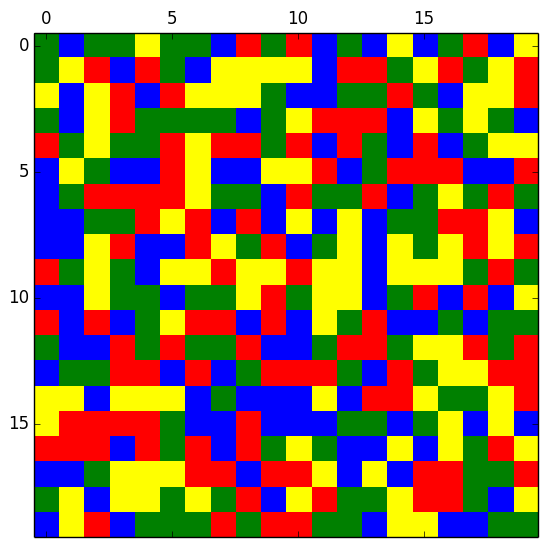
\includegraphics[width=0.45\textwidth]{plots/grid_initial.png}
	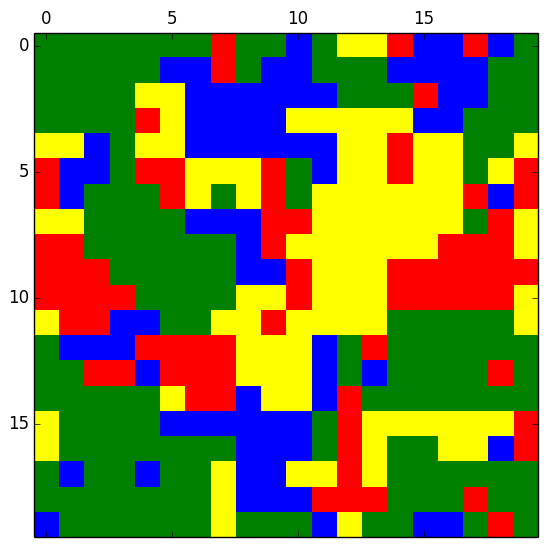
\includegraphics[width=0.45\textwidth]{plots/grid_b1_it401.png}
	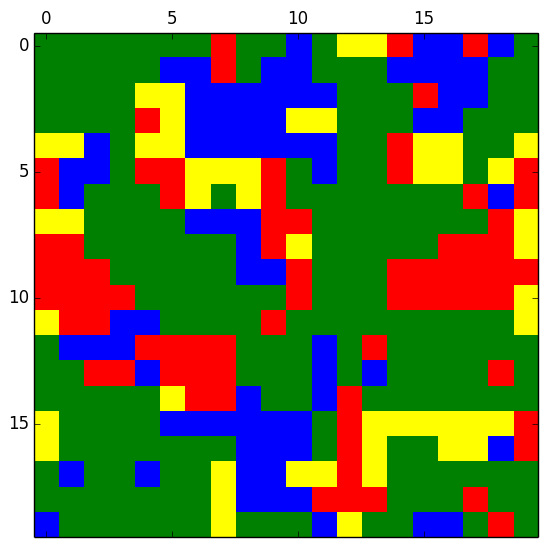
\includegraphics[width=0.45\textwidth]{plots/grid_b1_it402.png}
	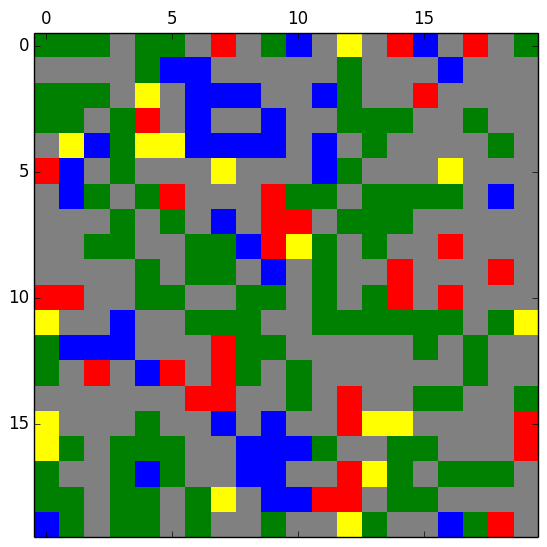
\includegraphics[width=0.45\textwidth]{plots/grid_b1_it402_missing.png}
	\caption{Potts model with $L = 4$ classes on an $N \times N = 20 \times 20$ dimensional grid. Topleft: random initialization; Topright: state after 401 iterations; bottomleft: state after 402 iterations of the Swendesn Wang Algorithm described in Section~\ref{swendsen_wang} with inverse temperature $\beta = 1$, note the flip of the central yellow cluster to green; bottomleft: randomly sampled $50\%$ missing values in grey.}
	\label{fig:potts_models}
\end{figure}
%
A GIF of SW sampling new observations in a Potts model in equilibrium can be found following this \href{https://github.com/maierhofert/2DPottsModel/blob/master/plots/grid_SW_equilibrium.gif}{\underline{link}}.


\subsection{Treatment of Missing Values}\label{treatment_of_missing_values}
The main goal of the project is to implement an algorithm to estimate a distribution over missing values by means of multiple imputation. The algorithms above for estimating the inverse temperature $\beta$ (Section~\ref{temperature_estimation}) 
and model sampling (Section~\ref{model_sampling}) assume a completely observed lattice $X$. The problem of estimating $\beta$ and calculating the model when missing values are present can be circumvented using a Gibbs sampler.
The Gibbs sampler for obtaining $M$ samples of the complete lattice works as follows: \\

\fbox{ \centering{
\parbox{0.9\textwidth}{\textbf{Multiple Imputation of Missing Values in Potts Model}
\begin{enumerate}
    \item Initialize all missing values $X_\text{miss}$ randomly from $\{1, 2, \ldots, L\}$ to obtain $X^0$
    \item Initialize $\beta^0$ % as %TODO 
    \item For $b$ in $1, 2, \ldots, B$ (burn-in):
    \begin{enumerate}[label*=\arabic*]
        \item Estimate $\beta^b$ from $X^{b-1}$ using MPLE \eqref{eq:beta_MPLE} \label{step:estimate_beta}
        \item Estimate $X^b_\text{miss}$ using SW \label{step:SW_miss} %TODO ref 
    \end{enumerate}
    \item For $m$ in $B + 1, B + 2, \ldots, B + M$ (sampling from distribution):
    \begin{enumerate}[label*=\arabic*]
        \item Estimate $\beta^m$ from $X^{m-1}$ using MCMC \eqref{eq:beta_MCMC} \label{step:estimate_beta2}
        \item Estimate $X^m_\text{miss}$ using SW \label{step:SW_miss2} %TODO ref
    \end{enumerate}
    \item Return $\left\{X^{B+1}, X^{B+2}, \ldots, X^{B+M}\right\}$
\end{enumerate}
}}}



\subsubsection{Missing Values in Temperature  Estimation}\label{missing_values_temperature}
The presence of missing values does not affect the estimation of the inverse temperature $\beta$ in Steps~\ref{step:estimate_beta} and~\ref{step:estimate_beta2}. The grid can be assumed to be fully observed and the Gibbs sampler ensures asymptotically unbiased estimates of $\beta$.
Initializing missing values randomly will result in a dramatical underestimation of the inverse temperature $\beta$. 
A long burnin could be necessary to move the grid into an equilibrium state with stable estimated $\beta$ when $\beta$ is large and/or a large number of values in the grid are missing, see Figure~\ref{fig:beta_missing}.
%
\begin{figure}
	\centering
	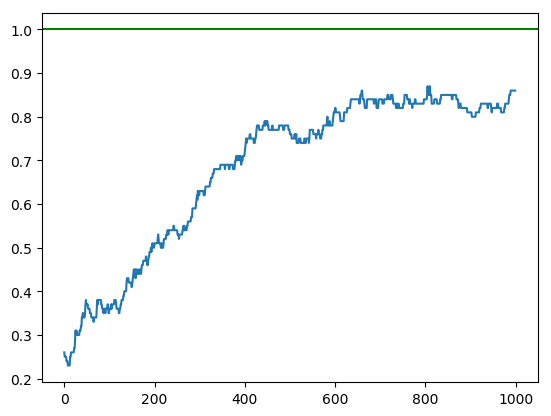
\includegraphics[width=0.7\textwidth]{plots/beta_b1_it500_missing.png}
	\caption{Burnin of the grid shown in the bottomleft of Figure~\ref{fig:potts_models} when missing values are initialized randomly. The plot shows the number of update steps on the $x$ axis vs. estimated $\beta$ on the $y$ axis. The true $\beta = 1$ is shown in green.}
	\label{fig:beta_missing}
\end{figure}
%


\subsubsection{Missing Values in Model Sampling}\label{missing_values_model_sampling}
Caution should be exercised in Step~\ref{step:SW_miss} as standard SW (Section~\ref{swendsen_wang}) will flip any $X_{ij} \in X$ regardless of whether are observed or missing. In this application, only missing pixels $X_{ij} \in X_\text{miss}$ should be flipped, as observed pixels $X_{kl} \in X_\text{obs}$ are, as the name suggests, observed and thus fixed. 
Proposing edge sets $E^*$ that result in clusters containing only unobserved pixels is non-trivial.\footnote{It is actually trivial to propose edge sets and thus clusters that contain only unobserved pixels, but I was unable to think of a clustering strategy for which the acceptance probabilities are not computationally complex, differ by proposed class, and are definitely not equal to 1.} 
An ad-hoc solution to this problem is keep proposing new edge sets and thus clusters until all observations in the cluster selected for flipping are unobserved. Then, the cluster can be flipped with probability 1.
% TODO write what it changes in the OG SW algorithm 
% This ad-hoc solutions 
%
A GIF of SW converging towards its equilibrium in the presence of missing values in a Potts model can be found following this \href{https://github.com/maierhofert/2DPottsModel/blob/master/plots/grid_missing_burnin.gif}{\underline{link}}.
%
A GIF of SW sampling observations for missing values in a Potts model in equilibrium can be found following this \href{https://github.com/maierhofert/2DPottsModel/blob/master/plots/grid_missing_equilibrium.gif}{\underline{link}}.
Note how the observed values in the grid never change.

\clearpage
\section{Future Research}\label{future_research}
There are a number of open research question that could not be addressed due to time constraints of this projects. 
The most important ones are:
\begin{itemize}
    \item How does the ratio of missing values affect the estimation of $\beta$? Undoubtedly, the variance will increase, but a bias towards smaller values of $\beta$ could be introduced, as fewer and fewer (in the extreme case no) neighboring pixels are observed. The estimator could also run into the risk of diverging for small proportions of observed values.
    \item It would be interesting to analyze the run-time of SW and the Gibbs sampler for missing values for varying proportions of missing values and $\beta$.
    \item Is there a way to create and flip clusters that only contain missing values?
\end{itemize}

%%%%%%%%%%%%%%%%%%%%%%%%%%%%%%%%%%%%%%%%%%%%%%%%%%%%%%%%%%%%%%%%%%%%%
\clearpage
\bibliographystyle{dcu} 
{\bibliography{bibliography.bib}}

%%%%%%%%%%%%%%%%%%%%%%%%%%%%%%%%%%%%%%%%%%%%%%%%%%%%%%%%%%%%%%%%%%%%%

\clearpage
\begin{appendix}
\appendix
\section*{Digital Appendix}
The Python implemention of all methods, figures, and GIFs presented in this report can be found in a publicly accessible  \href{https://github.com/maierhofert/2DPottsModel.git}{\underline{Github repository}}. The files \url{potts_SW_missing.py} and \url{animations.py} can be executed to recreate all figures and GIFs.
It also contains all figures, GIFs, and the Latex code used to generate this report.
\end{appendix}

\end{document}
